\documentclass[a4paper,10pt]{book}
\usepackage[centertags]{amsmath}
\usepackage{amscd}
\usepackage{amsthm}
\usepackage{amssymb}
\usepackage{enumerate}
\usepackage{multicol}
\usepackage[english,catalan,spanish]{babel}
\usepackage[all]{xy}
\usepackage{color}
\usepackage{tikz}
\usepackage{indentfirst}
\usepackage[utf8]{inputenc}
\usepackage[T1]{fontenc}
\linespread{1.1}
\setlength{\parskip}{10pt}
\usepackage[twoside,bindingoffset=1cm]{geometry}
\usepackage{lmodern}
\usepackage[x11names, dvipsnames, table]{xcolor}
\definecolor{ubblue}{HTML}{0059A2}
\usepackage[colorlinks=true, linkcolor=black, citecolor=ubblue, urlcolor=ubblue]{hyperref}
\usepackage{cleveref}
\usepackage[protrusion=true,expansion=true]{microtype}
\usepackage{cite}


%% Custom packages


%%%%%%%%%%%%%%%%%%%%%%%%%%%%%%%%%%%%%%%%%%%%%%%%%%%%%%%%%%%%%%%%%%%%%%%%%%%
%%%% local definitions for this paper
%%%%%%%%%%%%%%%%%%%%%%%%%%%%%%%%%%%%%%%%%%%%%%%%%%%%%%%%%%%%%%%%%%%%%%%%%%%


%%%%%%%%%%%%%%%%%%%%%% aix{\`o} pels headings %%%%%%%%%%%%%%%%%%%%%%%%
\usepackage{fancyhdr}
\pagestyle{fancy}
\renewcommand{\chaptermark}[1]{\markboth{#1}{}}
\renewcommand{\sectionmark}[1]{\markright{\thesection\ #1}}
\fancyhf{} \fancyhead[LE,RO]{\bfseries\thepage}
\fancyhead[LO]{\bfseries\rightmark} \fancyhead[RE]{\bfseries\leftmark}

\def\paginaenblanc{\newpage%
\thispagestyle{empty}%
\vspace*{2cm}%
\newpage%
\thispagestyle{empty}%
}


%%%%%%%%%%%%%%%%%%%%%%%%%%%%%%%%%%%%%%%%%%%%%%%%%%%%%%%%%%%%%%%%%%%%%%%%%
% aux commands
%%%%%%%%%%%%%%%%%%%%%%%%%%%%%%%%%%%%%%%%%%%%%%%%%%%%%%%%%%%%%%%%%%%%%%%%%
%==========================================================================
% macros to support private authors' notes
%==========================================================================
\newif\ifprivate
\privatetrue
\def\xbar{\vskip0.09in\hrule\vskip0.06in}
\def\private#1{\ifprivate \xbar {\em #1} \xbar
\else \fi}
\def\huh{\ifprivate ??? \marginpar{\Huge ???}
\else \fi}
\def\???{\ifprivate {\bf {???}} \marginpar{\begin{center}{\Huge {\bf ?}}\end{center}}
\else \fi}
%\def\???{\ifprivate {\bf {???}} \marginpar{{\Huge {\bf ?}}}
%\else \fi}
\marginparsep1mm
\def\nota#1{\ifprivate  $\clubsuit$ \marginpar{\parbox[t]{2.4cm}{\begin{center}\tiny #1\end{center}}}
\else \fi}
\def\comment#1{\ifprivate \marginpar{\parbox[t]{2.4cm}{\begin{center}\tiny #1\end{center}}}
\else \fi}
%\def\nota#1{\ifprivate  $\clubsuit$ \marginpar{\parbox[t]{1.8cm}{\tiny #1}}
%\else \fi}
\def\privateeject{\ifprivate\eject\fi}
%\def\???{{\bf {???}} \marginpar{{\Huge {\bf ?}}} }
%%%%%%%%%%%%%%%%%%%%%%%%%%%%%%%%%%%%%%%%%%%%%%%%%%%%%%%%%%%%%%%%%%%%%%%%%%

%%%%%%%%%%%%%%%%%%%%%%%%%%%%%%%%%%%%%%%%%%%%%%%%%%%%%%%%%%%%%%%%%%%%%%%%
%%%%%%%%%%%%%%%%%%%%%%%%%%%%%%%%%%%%%%%%%%%%%%%%%%%%%%%%%%%%%%%%%%%%%%%%
\begin{document}

\pagestyle{empty}

\begin{titlepage}
\begin{center}
\begin{figure}[htb]
\begin{center}

\includegraphics[width=6cm]{assets/ub_color.pdf}
\end{center}
\end{figure}

\def\worktitle{Development of an AI-Based Tool for Molecular Subtype Classification of Invasive Ductal Breast Carcinoma Using Mammography}

\textbf{\LARGE Treball final de grau} \\
\vspace*{.5cm}
\textbf{\LARGE GRAU D'ENGINYERIA INFORM\`{A}TICA } \\
\vspace*{.5cm}
\textbf{\LARGE Facultat de Matem\`atiques i Inform\`atica\\ Universitat de Barcelona} \\
\vspace*{1.0cm}
\rule{16cm}{0.1mm}\\
\begin{Huge}
\textbf{Development of an AI-Based Tool for Molecular Subtype Classification of Invasive Ductal Breast Carcinoma Using Mammography} \\
\end{Huge}
\rule{16cm}{0.1mm}\\

\vspace{1cm}

\begin{flushright}


\vspace*{2.5cm}

\hfill

\renewcommand{\arraystretch}{1.5}
\begin{tabular}{ll}
\textbf{\small Autor:} & \textbf{\small David Bland\'on T\'orrez } \\
\textbf{\small Director:} & \textbf{\small Dr. Oliver D\'iaz Montesdeoca } \\
\textbf{\small Realitzat a:} & \textbf{\small  Departament de Matem\`{a}tiques i  Inform\`{a}tica  } \\
\textbf{\small Barcelona,} & \textbf{\small \today }
\end{tabular}

\end{flushright}

\end{center}

\end{titlepage}

%%%%%%%%%%%%%%%%%%%%%%%%%%%%%%%%%%%%%%%%%%%%%%%%%%%%%%%%%%%%%%%%%%%%%%%%%
\newpage
\selectlanguage{english}
\noindent \textbf{\large Abstract}

// TODO

%%%%%%%%%%%%%%%%%%%%%%%%%%%%%%%%%%%%%%%%%%%%%%%%%%%%%%%%%%%%%%%%%%%%%%%%%

%%%%%%%%%%%%%%%%%%%%%%%%%%%%%%%%%%%%%%%%%%%%%%%%%%%%%%%%%%%%%%%%%%%%%%%%%
\newpage
\selectlanguage{spanish}
\noindent \textbf{\large Resumen}

// TODO

%%%%%%%%%%%%%%%%%%%%%%%%%%%%%%%%%%%%%%%%%%%%%%%%%%%%%%%%%%%%%%%%%%%%%%%%%

%%%%%%%%%%%%%%%%%%%%%%%%%%%%%%%%%%%%%%%%%%%%%%%%%%%%%%%%%%%%%%%%%%%%%%%%%
\newpage
\selectlanguage{catalan}
\noindent \textbf{\large Resum}

// TODO

%%%%%%%%%%%%%%%%%%%%%%%%%%%%%%%%%%%%%%%%%%%%%%%%%%%%%%%%%%%%%%%%%%%%%%%%%
\newpage
\selectlanguage{english}
\noindent \textbf{\large Acknowledgements}

// TODO
%%%%%%%%%%%%%%%%%%%%%%%%%%%%%%%%%%%%%%%%%%%%%%%%%%%%%%%%%%%%%%%%%%%%%%%%%
\selectlanguage{english}
\pagenumbering{roman} \setcounter{page}{0}
\let\cleardoublepage\clearpage
\tableofcontents
\newpage \thispagestyle{empty}
%%%%%%%%%%%%%%%%%%%%%%%%%%%%%%%%%%%%%%%%%%%%%%%%%%%%%%%%%%%%%%%%%%%%%%%%%

\pagestyle{fancy}
\markboth{Introducción}{Introducción}
\newpage \thispagestyle{empty}
%%%%%%%%%%%%%%%%%%%%%%%%%%%%%%%%%%%%%%%%%%%%%%%%%%%%%%%%%%%%%%%%%%%%%%%%%
\mainmatter
\chapter{Introduction}
\section{Problem Context}

Breast cancer has become one of the leading causes of mortality among women and represents the type of cancer with the highest incidence in this population. It is estimated that, on average, one in twenty women worldwide will be diagnosed with this disease during their lifetime \cite{kim_global_2025}. Recent projections suggest that if current trends continue, by the year 2050, approximately 3.2 million new cases and 1.1 million deaths associated with this pathology will be recorded, with a particularly significant impact in countries with a low Human Development Index (HDI) \cite{kim_global_2025}.

Against this backdrop, early diagnostic techniques and tools play a fundamental role in improving patient prognosis and survival rates \cite{wang_early_2017}. However, breast cancer is a heterogeneous disease\footnote{Cellular diversity either within a single tumor (intratumoral heterogeneity) or among different tumors in the same individual (intertumoral heterogeneity).} that can be classified into various subtypes according to clinical and especially molecular characteristics. The international guidelines from the 2013 St. Gallen Consensus \cite{goldhirsch_personalizing_2013} recognize four main subtypes based on hormone receptor status (estrogen, progesterone) and the proliferation marker Ki67: Luminal A, Luminal B, HER2-positive (HER2-enriched), and Triple Negative (see Figure \ref{fig:subtypes}). This classification has direct clinical implications, as prognosis, treatment response, and therapeutic options largely depend on the molecular subtype to which the tumor belongs.

Currently, tumor molecular characterization is primarily performed through biopsy, an invasive and costly procedure that may need to be repeated, potentially delaying treatment initiation and increasing the clinical, physical, and emotional burden on patients. Therefore, there is a growing need to develop non-invasive, accessible, and efficient methods that can perform this task reliably. In this regard, mammography stands out as a key tool, being a non-invasive, low-cost, and widely used technique for early breast cancer detection.

\begin{figure}
    \centering
    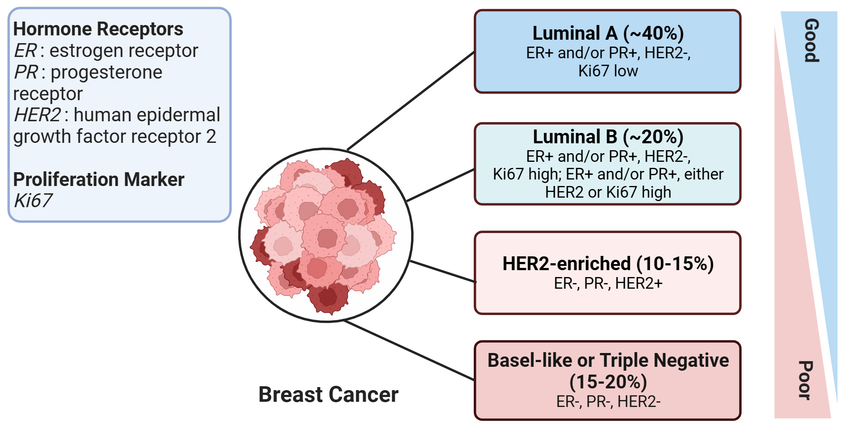
\includegraphics[width=0.8\linewidth]{reports/assets/subtypes.png}
    \caption{The 4 molecular subtypes of breast cancer and their prevalence percentage \cite{harnessing_2024}}
    \label{fig:subtypes}
\end{figure}

In recent years, advances in artificial intelligence (AI), along with the increasing availability of data and more efficient computational capabilities, have driven the development of deep learning (DL) models for tasks such as classification, detection, and prediction of breast cancer, among other diseases. Several studies have demonstrated that these systems can match or even surpass the performance of human experts or traditional CAD (Computer-Aided Diagnosis) systems in these tasks \cite{mckinney_international_2020,pattanaik_breast_2022,meenalochini_deep_2024,hussain_performance_2025}, highlighting the significant impact of this technology and its potential clinical benefit for patient care.

Recent studies have explored the classification of molecular subtypes from mammographic images. Mota et al. (2024) \cite{mota_breast_2024} addressed this task using mammographic images exclusively, achieving an AUC of 60.62\% in multiclass classification with a ResNet101 architecture. Similarly, Rabah et al. (2025) \cite{ben_rabah_multimodal_2025} reported an AUC of 63.79\% using an Xception-based model and further proposed a multimodal approach integrating clinical metadata, which increased performance to 88.87\% AUC. Although the results obtained in unimodal scenarios remain modest and below the clinical utility threshold (\textasciitilde80\% AUC), these studies demonstrate the potential of imaging as a diagnostic source and reinforce the need for continued research to improve the precision and clinical utility of these models.

This study proposes an unimodal approach based exclusively on mammograms from the publicly available CMMD dataset \cite{cai_online_2023}, aiming to compare the performance of state-of-the-art Transformer-based architectures—Vision Transformer (ViT), Shifted-Windows Transformer (SwinT), and Multi-Axis Vision Transformer (MaxViT)—against a traditional deep convolutional neural network (CNN) baseline. Although multimodal models often achieve higher performance by integrating complementary clinical data, focusing solely on mammographic images has high practical value, especially in resource-limited settings or where clinical data standardization is not guaranteed. Recent studies have shown that Transformers outperform CNNs in accuracy and robustness for medical classification tasks due to their self-attention mechanisms, which allow them to capture global spatial relationships within the image \cite{mauricio_comparing_2023}. Based on these capabilities, it is hypothesized that the Transformer architectures analyzed could achieve superior performance in molecular subtype classification, even under an unimodal approach.

Ultimately, this work aims to contribute to the development of non-invasive diagnostic tools by systematically evaluating Transformer models, with the goal of advancing toward automated, accessible, and efficient molecular characterization of breast cancer—particularly in contexts where biopsy is not an immediate option—thereby improving equitable access to diagnosis and reducing therapeutic intervention delays.

\section{Objectives}

The main objective of this study is to develop a deep learning model capable of classifying molecular subtypes of breast cancer using only mammographic images from the \textit{Chinese Mammography Database} (CMMD), without relying on clinical metadata or auxiliary annotations. This task poses significant challenges, such as class imbalance between molecular subtypes, scarcity of labeled data, and the absence of region-of-interest annotations in the images, which hinder effective learning and may limit AI model performance in medical applications.

To address these challenges, the performance of various modern Transformer-based architectures, specifically, Vision Transformer (ViT), Shifted-Window Transformer (SwinT), and Multi-Axis Vision Transformer (MaxViT), will be systematically evaluated and compared to traditional convolutional neural network models. The focus on these architectures lies in their ability to capture global relationships and complex patterns in images through attention mechanisms, which is particularly relevant for identifying subtle features associated with molecular heterogeneity in mammograms.

Extensive experiments will be conducted, incorporating adaptive data augmentation strategies (rotations, flips, and intensity transformations specific to mammography), oversampling techniques, and weighted loss functions to tackle class imbalance. Performance will be evaluated using robust metrics such as weighted F1-score, area under the ROC curve (AUC-ROC), and balanced accuracy, enabling an objective comparison across architectures.

With the results obtained, a comparative analysis will be carried out against previous studies that have addressed the same problem.

Additionally, an explainability analysis of the best-performing model will be conducted through the generation of attention maps and Gradient-weighted Class Activation Mapping (Grad-CAM) techniques. This will help identify the mammographic regions that contribute significantly to the model's decisions, facilitating clinical validation and providing insights into the visual patterns associated with each molecular subtype.

... // TODO: Develop conclusion and statistical analysis (p-values)

\section{Planning}

\subsection{Tasks to Develop}

// TODO

\subsection{Schedule}

// TODO

%%%%%%%%%%%%%%%%%%%%%%%%%%%%%%%%%%%%%%%%%%%%%%%%%%%%%%%%%%%%%%%%%%%%%%%%%

\chapter{Background}
\section{Breast Cancer}
\section{Molecular Subtypes}
\section{Screening Process}
\section{Mammography}

\chapter{Technology Review}

\chapter{Materials and Methods}
\section{CMMD Dataset}
\section{Image Preprocessing}

\chapter{Results and Discussion}
\section{Results}

\chapter{Conclusions and Future Work}

%%%%%%%%%%%%%%%%%%%%%%%%%%%%%%%%%%%%%%%%%%%%%%%%%%%%%%%%%%%%%%%%%%%%%%%%%
\backmatter
\selectlanguage{english}
\addcontentsline{toc}{chapter}{Bibliography}
\bibliographystyle{ieeetr}
\bibliography{references}

\end{document}
